

\tikzset{every picture/.style={line width=0.75pt}} %set default line width to 0.75pt        

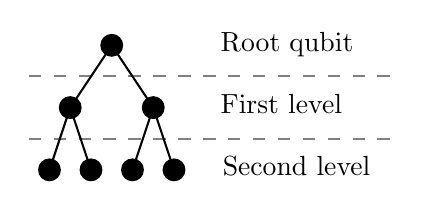
\begin{tikzpicture}[x=0.75pt,y=0.75pt,yscale=-1,xscale=1]
%uncomment if require: \path (0,300); %set diagram left start at 0, and has height of 300

%Straight Lines [id:da8426905590991587] 
\draw [color={rgb, 255:red, 128; green, 128; blue, 128 }  ,draw opacity=1 ] [dash pattern={on 4.5pt off 4.5pt}]  (60,85) -- (240,85) ;
%Straight Lines [id:da5406148798931413] 
\draw [color={rgb, 255:red, 128; green, 128; blue, 128 }  ,draw opacity=1 ] [dash pattern={on 4.5pt off 4.5pt}]  (60,55) -- (240,55) ;
%Straight Lines [id:da0310472865739988] 
\draw    (80,70) -- (90,100) ;
%Straight Lines [id:da44724908569705224] 
\draw    (80,70) -- (100,40) ;
%Shape: Circle [id:dp9646050192410193] 
\draw  [fill={rgb, 255:red, 0; green, 0; blue, 0 }  ,fill opacity=1 ] (95,40) .. controls (95,37.24) and (97.24,35) .. (100,35) .. controls (102.76,35) and (105,37.24) .. (105,40) .. controls (105,42.76) and (102.76,45) .. (100,45) .. controls (97.24,45) and (95,42.76) .. (95,40) -- cycle ;
%Shape: Circle [id:dp9987430184128605] 
\draw  [fill={rgb, 255:red, 0; green, 0; blue, 0 }  ,fill opacity=1 ] (105,100) .. controls (105,97.24) and (107.24,95) .. (110,95) .. controls (112.76,95) and (115,97.24) .. (115,100) .. controls (115,102.76) and (112.76,105) .. (110,105) .. controls (107.24,105) and (105,102.76) .. (105,100) -- cycle ;
%Shape: Circle [id:dp5327923177036115] 
\draw  [fill={rgb, 255:red, 0; green, 0; blue, 0 }  ,fill opacity=1 ] (125,100) .. controls (125,97.24) and (127.24,95) .. (130,95) .. controls (132.76,95) and (135,97.24) .. (135,100) .. controls (135,102.76) and (132.76,105) .. (130,105) .. controls (127.24,105) and (125,102.76) .. (125,100) -- cycle ;
%Shape: Circle [id:dp07874792740386194] 
\draw  [fill={rgb, 255:red, 0; green, 0; blue, 0 }  ,fill opacity=1 ] (115,70) .. controls (115,67.24) and (117.24,65) .. (120,65) .. controls (122.76,65) and (125,67.24) .. (125,70) .. controls (125,72.76) and (122.76,75) .. (120,75) .. controls (117.24,75) and (115,72.76) .. (115,70) -- cycle ;
%Shape: Circle [id:dp827553292195197] 
\draw  [fill={rgb, 255:red, 0; green, 0; blue, 0 }  ,fill opacity=1 ] (65,100) .. controls (65,97.24) and (67.24,95) .. (70,95) .. controls (72.76,95) and (75,97.24) .. (75,100) .. controls (75,102.76) and (72.76,105) .. (70,105) .. controls (67.24,105) and (65,102.76) .. (65,100) -- cycle ;
%Shape: Circle [id:dp9737971224660668] 
\draw  [fill={rgb, 255:red, 0; green, 0; blue, 0 }  ,fill opacity=1 ] (85,100) .. controls (85,97.24) and (87.24,95) .. (90,95) .. controls (92.76,95) and (95,97.24) .. (95,100) .. controls (95,102.76) and (92.76,105) .. (90,105) .. controls (87.24,105) and (85,102.76) .. (85,100) -- cycle ;
%Shape: Circle [id:dp3888180938045467] 
\draw  [fill={rgb, 255:red, 0; green, 0; blue, 0 }  ,fill opacity=1 ] (75,70) .. controls (75,67.24) and (77.24,65) .. (80,65) .. controls (82.76,65) and (85,67.24) .. (85,70) .. controls (85,72.76) and (82.76,75) .. (80,75) .. controls (77.24,75) and (75,72.76) .. (75,70) -- cycle ;
%Straight Lines [id:da09087177582110562] 
\draw    (80,70) -- (70,100) ;
%Straight Lines [id:da9701309593546271] 
\draw    (100,40) -- (120,70) ;
%Straight Lines [id:da7485547301936679] 
\draw    (110,100) -- (120,70) ;
%Straight Lines [id:da005037302745795835] 
\draw    (120,70) -- (130,100) ;

% Text Node
\draw (151,32) node [anchor=north west][inner sep=0.75pt]   [align=left] {Root qubit};
% Text Node
\draw (151,62) node [anchor=north west][inner sep=0.75pt]   [align=left] {First level};
% Text Node
\draw (152,92) node [anchor=north west][inner sep=0.75pt]   [align=left] {Second level};


\end{tikzpicture}